% -*- mode: LaTeX; TeX-PDF-mode: t; -*- # Tell emacs the file type (for syntax)
% -*- mode: LaTeX; TeX-PDF-mode: t; -*- # Tell emacs the file type (for syntax)
% LaTeX path to the root directory of the current project, from the directory in which this file resides
% and path to econtexPaths which defines the rest of the paths like \FigDir
\providecommand{\econtexRoot}{}\renewcommand{\econtexRoot}{.}
\providecommand{\econtexPaths}{}\renewcommand{\econtexPaths}{\econtexRoot/Resources/econtexPaths}
% -*- mode: LaTeX; TeX-PDF-mode: t; -*- 
% The \commands below are required to allow sharing of the same base code via Github between TeXLive on a local machine and Overleaf (which is a proxy for "a standard distribution of LaTeX").  This is an ugly solution to the requirement that custom LaTeX packages be accessible, and that Overleaf prohibits symbolic links
\providecommand{\packages}{\econtexRoot/Resources/texmf-local/tex/latex}
\providecommand{\econtex}{\packages/econtex}
\providecommand{\econark}{\econtexRoot/Resources/texmf-local/tex/latex/econark}
\providecommand{\econtexSetup}{\econtexRoot/Resources/texmf-local/tex/latex/econtexSetup}
\providecommand{\econtexShortcuts}{\econtexRoot/Resources/texmf-local/tex/latex/econtexShortcuts}
\providecommand{\econtexBibMake}{\econtexRoot/Resources/texmf-local/tex/latex/econtexBibMake}
\providecommand{\econtexBibStyle}{\econtexRoot/Resources/texmf-local/bibtex/bst/econtex}
\providecommand{\econtexBib}{economics}
\providecommand{\notes}{\econtexRoot/Resources/texmf-local/tex/latex/handout}
\providecommand{\handoutSetup}{\econtexRoot/Resources/texmf-local/tex/latex/handoutSetup}
\providecommand{\handoutShortcuts}{\econtexRoot/Resources/texmf-local/tex/latex/handoutShortcuts}
\providecommand{\handoutBibMake}{\econtexRoot/Resources/texmf-local/tex/latex/handoutBibMake}
\providecommand{\handoutBibStyle}{\econtexRoot/Resources/texmf-local/bibtex/bst/handout}

\providecommand{\FigDir}{\econtexRoot/Figures}
\providecommand{\CodeDir}{\econtexRoot/Code}
\providecommand{\DataDir}{\econtexRoot/Data}
\providecommand{\SlideDir}{\econtexRoot/Slides}
\providecommand{\TableDir}{\econtexRoot/Tables}
\providecommand{\ApndxDir}{\econtexRoot/Appendices}

\providecommand{\ResourcesDir}{\econtexRoot/Resources}
\providecommand{\rootFromOut}{..} % APFach back to root directory from output-directory
\providecommand{\LaTeXGenerated}{\econtexRoot/LaTeX} % Put generated files in subdirectory
\providecommand{\econtexPaths}{\econtexRoot/Resources/econtexPaths}
\providecommand{\LaTeXInputs}{\econtexRoot/Resources/LaTeXInputs}
\providecommand{\LtxDir}{LaTeX/}
\providecommand{\EqDir}{\econtexRoot/Equations} % Put generated files in subdirectory

\providecommand{\local}{\LaTeXInputs/local}

\documentclass[titlepage,abstract]{\econtex}
\newcommand{\texname}{cctwMoM}
\usepackage{import}
\usepackage{\econark}
\usepackage{\LaTeXInputs/SolvingMicroDSOPs}
 

% RiskyR
\provideboolean{RiskyR}
\setboolean{RiskyR}{true}
\setboolean{RiskyR}{false}
\newcommand{\IfRiskyR}{\ifthenelse{\boolean{RiskyR}}}

% Include permanent shocks?
\provideboolean{PermShkVersion}
%\setboolean{PermShkVersion}{true}
\setboolean{PermShkVersion}{false}
\newcommand{\PermShkOn}{\ifthenelse{\boolean{PermShkVersion}}}

% MPCMatch
\provideboolean{MPCMatchVersion}
\setboolean{MPCMatchVersion}{false}
\newcommand{\MPCMatch}{\ifthenelse{\boolean{MPCMatchVersion}}}

\provideboolean{MoMVersion}
\setboolean{MoMVersion}{true}
\newcommand{\MoM}{\ifthenelse{\boolean{MoMVersion}}}

\provideboolean{ctwVersion}
\setboolean{ctwVersion}{true}
\newcommand{\ctw}{\ifthenelse{\boolean{ctwVersion}}}


\usepackage{\econtexSetup}\usepackage{\econtexShortcuts}
\write18{rm    ./Figures/List.tex }
\write18{touch ./Figures/List.tex }

\hypersetup{colorlinks=true,
            pdfauthor={Christopher D. Carroll <ccarroll@jhu.edu>, Kiichi Tokuoka <ktokuoka <ktokuoka@imf.org>, Weifeng Wu <wwu19@jhu.edu> },
            pdftitle={The Method of Moderation},
            pdfsubject={Dynamic Stochastic Optimization Theory; Lecture Notes},
            pdfkeywords={Numerical Methods, Software},
            pdfproducer = {LaTeX with hyperref and thumbpdf},
            pdfcreator = {pdflatex}
            }

\begin{verbatimwrite}{./\texname.title}
The Method of Moderation
\end{verbatimwrite}

\bibliographystyle{\econtexBibStyle}\begin{document}

%\hfill {\small WuW Thesis Version}

\title{The Method of Moderation}

\author{Christopher D. Carroll\num \\ {\small JHU}
  \and
  Karsten Chipeniuk \\ {\small RBNZ}
  \and 
Kiichi Tokuoka\num \\ {\small ECB}
\and
Weifeng Wu\num \\ {\small Fannie Mae}
}

\keywords{Dynamic Stochastic Optimization}
\jelclass{FillInLater}

\maketitle

\begin{abstract}
  In a risky world, a pessimist assumes the worst will happen.  Someone who ignores risk altogether is an optimist.  Consumption decisions are mathematically simple for both the pessimist and the optimist because both behave as if they live in a riskless world.  A realist (that is, someone who wants to respond optimally to risk) faces a much more difficult problem, but (under standard conditions) will choose a level of spending somewhere between pessimist's and the optimist's.  We use this fact to redefine the space in which the realist searches for optimal consumption rules.  The resulting solution accurately represents the numerical consumption rule over the entire interval of feasible wealth values with remarkably few computations.
\end{abstract}

% \begin{small}
% \parbox{\textwidth}{
% \begin{center}
% \begin{tabbing}
% \texttt{Archive:~} \= \= \url{http://econ.jhu.edu/people/ccarroll/papers/ctwMoM.pdf} \kill \\  % This line establishes the locations of the tabs, but is not printed because of the \kill directive
% \texttt{~~~~PDF:~} \> \> \url{http://econ.jhu.edu/people/ccarroll/papers/ctwMoM.pdf} \\
% \texttt{~Slides:~} \> \> \url{http://econ.jhu.edu/people/ccarroll/papers/ctwMoM-Slides.pdf} \\
% \texttt{~~~~Web:~} \> \> \url{http://econ.jhu.edu/people/ccarroll/papers/ctwMoM/} \\
% \texttt{Archive:~} \> \> \url{http://econ.jhu.edu/people/ccarroll/papers/ctwMoM.zip} \\
% %\texttt{~~~~~~~~~} \> \> \textit{(Contains data and estimation software producing paper's results)}
% \end{tabbing}
% \end{center}
% }
% \end{small}

\begin{authorsinfo}
\name{Carroll: Department of Economics, Johns Hopkins University, Baltimore, MD, \url{http://econ.jhu.edu/people/ccarroll/}, \href{mailto:ccarroll@jhu.edu}{\texttt{ccarroll@jhu.edu}}}
\name{Tokuoka: International Monetary Fund, Washington, DC, \href{mailto:ktokuoka@imf.org}{\texttt{ktokuoka@imf.org}}}
\name{Wu: Weifeng Wu, Fanie Mae, Washington DC, \href{mailto:weifeng\_wu@fanniemae.com}.}
\end{authorsinfo}

\thanks{The views presented in this paper are those of the authors, and should not be attributed to the International Monetary Fund, its Executive Board, or management, or to the European Central Bank.}

\thispagestyle{empty}


\pagebreak\newpage


\renewcommand{\DiscAlt}{\beta} % Erase the distinction between the alternative and the standard discount factor

\hypertarget{Introduction}{}
\section{Introduction}\label{sec:Intro}

Solving a consumption, investment, portfolio choice, or similar
intertemporal optimization problem using numerical methods generally
requires the modeler to choose how to represent a policy or value
function.  In the stochastic case, where analytical solutions are
generally not available, a common approach is to use low-order
polynominal splines that exactly match the function (and maybe some
derivatives) at a finite set of gridpoints, and then to assume that
interpolated or extrapolated versions of that 
spline represent the function well at the continuous infinity of unmatched points.

This paper argues that a better approach in the standard consumption 
problem is to rely upon the fact that without uncertainty, the optimal consumption
function has a simple analytical solution.  The key insight is that,
under standard assumptions, the consumer who faces an uninsurable
labor income risk will consume less than a consumer with the same path
for expected income but who does not perceive any uncertainty as being
attached to that future income.  The `realistic' consumer, who \textit{
  does} perceive the risks, will engage in `precautionary saving,' so
the perfect foresight riskless solution provides an upper bound to the
solution that will actually be optimal.  A lower bound is provided by
the behavior of a consumer who has the subjective belief that the
future level of income will be the worst that it can possibly be.
This consumer, too, behaves according to the convenient analytical perfect
foresight solution, but his certainty is that of a pessimist 
perfectly confident in his pessimism.

Using results from \cite{BufferStockTheory}, we show how to use these
upper and lower bounds to tightly constrain the shape and
characteristics of the solution to problem of the `realist.'  Imposition
of these constraints can clarify and speed the solution of the realist's problem.

After showing how to use the method in the baseline case, we show how
refine it to encompass an even tighter theoretical bound\IfRiskyR{, and 
how to extend it to solve a problem in which the consumer faces both 
labor income risk and rate-of-return risk.}{.}  

\hypertarget{The-Realists-Problem}{}
\section{The Realist's Problem}

We assume that truly optimal behavior in the problem facing the consumer who understands all his risks is captured by
\import{./Equations/}{MaxProb.tex}
%\write18{if [ ! -f \texname.bib ]; then touch \texname.bib  ; fi}\write18{if [ ! -f \texname-Add.bib ]; then touch \texname-Add.bib  ; fi}\bibliography{economics,\texname,\texname-Add}\end{document}\endinput
subject to
\import{./Equations/}{DBCLevelStart.tex}
where
\import{./Equations/}{Defns.tex}
and the exogenous variables evolve according to 
\import{./Equations/}{ExogVars.tex}

It turns out (see \cite{SolvingMicroDSOPs} for a proof) that this
problem can be rewritten in a more convenient form in
which choice and state variables are normalized by the level of
permanent income, e.g., using nonbold font for normalized variables, $\mRat_{t}=\cLev_{t}/\pLev_{t}$.  When that is
done, the Bellman equation for the transformed version of the consumer's problem is 
\import{./Equations/}{vNormed.tex}
and because we have not imposed a liquidity constraint, the solution 
satisfies the Euler equation
\import{./Equations/}{cEuler.tex}

For the remainder of the paper we will assume that permanent income $\pLev_{t}$ 
grows by a constant factor $\PermGroFac$ and is not subject to stochastic shocks.  
(The generalization to the case with permanent shocks is 
straightforward.)



\hypertarget{Benchmark}{}
\section{Benchmark: The Method of Endogenous Gridpoints}

For comparison to our new solution method, we use the endogenous
gridpoints solution to the microeconomic problem presented in
\cite{carrollEGM}.  That method computes the level of
consumption at a set of gridpoints for market resources $\mRat$ that
are determined endogenously using the Euler equation.  The consumption
function is then constructed by linear interpolation among the
gridpoints thus found.

\cite{SolvingMicroDSOPs} describes a specific calibration of the model and
constructs a solution using five gridpoints chosen to 
capture the structure of the consumption function reasonably well at values of
$\mRat$ near the infinite-horizon target value.  (See those notes for details).  

\import{\econtexRoot}{cctwMoM/EndogGptsProbs.tex}

\hypertarget{The-Method-Of-Moderation}{}
\section{The Method of Moderation}

\hypertarget{The-Optimist-The-Pessimist-and-the-Realist}{}
\subsection{The Optimist, the Pessimist, and the Realist}

\hypertarget{The-Consumption-Function}{}
\subsubsection{The Consumption Function}

\import{\econtexRoot/}{cctwMoM/MoM-Prelims.tex}
\import{./Equations/}{cFuncAbove.tex} 
\import{\econtexRoot/}{cctwMoM/MoM-Words.tex}

\import{./Figures/}{IntExpFOCInvPesReaOptNeedHiPlot.tex}
\import{\econtexRoot/}{cctwMoM/MoM-Words-Rest.tex}
\import{./Equations/}{MoM-Inequalities.tex}
\import{\econtexRoot/}{cctwMoM/MoM-Inequalities-Describe.tex}
\import{./Equations/}{MoM-KoppaOfMu.tex}
\import{\econtexRoot/}{cctwMoM/MoM-KoppaOfMu-Describe.tex}
\import{./Equations/}{cFuncHi.tex}
\import{\econtexRoot/}{cctwMoM/MoM-End.tex}

\subsubsection{The Value Function}

\import{\econtexRoot/}{cctwMoM/value-Intro.tex} % Can't nest verbatimwrites so must split value.tex up into parts
\import{./Equations/}{vFuncPF.tex} % This is the perfect foresight solution 
\import{\econtexRoot/}{cctwMoM/value-Rest.tex} % Remainder of the text

\section{Extensions}

\subsection{A Tighter Upper Bound}
\import{\econtexRoot/}{cctwMoM/Tighter.tex}
\import{./Equations/}{mtCusp.tex}
\import{./Equations/}{TighterUpperBound.tex}
\import{./Equations/}{koppaLo.tex}
\import{\econtexRoot/}{cctwMoM/TighterThreeFuncs.tex}
\import{./Equations/}{TighterThreeEqns.tex}
\import{\econtexRoot/}{cctwMoM/TighterThreeFuncsExplain.tex}

\begin{figure}
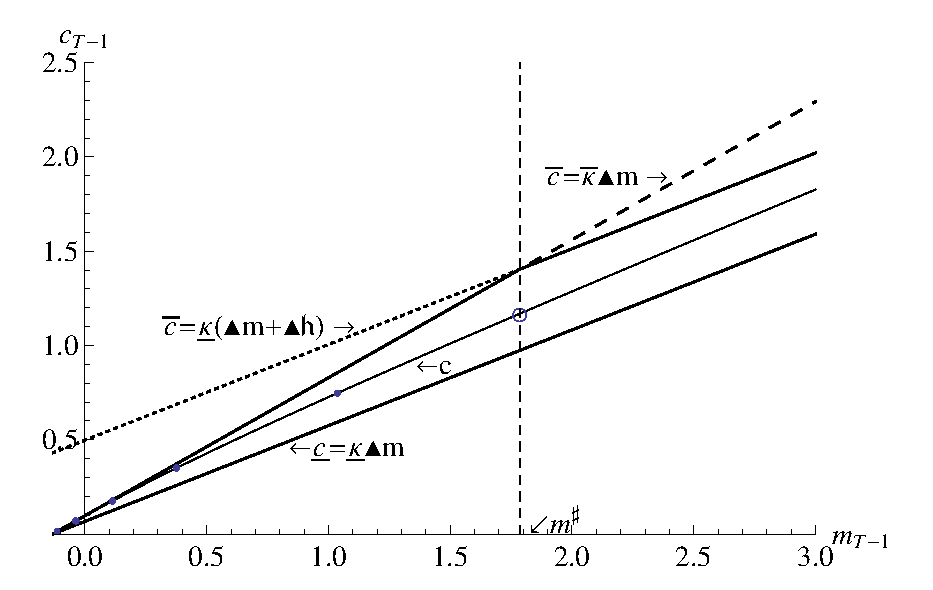
\includegraphics[width=6in]{./Figures/IntExpFOCInvPesReaOptNeed45Plot}
\end{figure}

\IfRiskyR{
  \hypertarget{Stochastic-Rate-of-Return}{}
\subsection{Stochastic Rate of Return}
\import{\econtexRoot/}{cctwMoM/StochasticR-Intro.tex} 

The easiest case is where the interest factor is i.i.d.,
\import{./Equations/}{distRisky.tex} 
\noindent because in this case \cite{merton:restat} and \cite{samuelson:portfolio} showed
that for a consumer without labor income (or with perfectly forecastable labor income) the consumption
function is linear, with an MPC\footnote{See \handoutC{CRRA-RateRisk} for a derivation.}
\import{\econtexRoot/}{cctwMoM/R-IID-MertonSamuelson.tex} 
\import{\econtexRoot/}{cctwMoM/R-AR1.tex} 
}{}

%\subsection{Habits}


\section{Conclusion}

The method proposed here is not universally applicable.  For example,
the method cannot be used for problems for which upper and lower
bounds to the `true' solution are not known.  But many problems do 
have obvious upper and lower bounds, and in those cases (as in the 
consumption example used in the paper), the method may result in 
substantial improvements in accuracy and stability of solutions.



\vfill\clearpage
\write18{if [ ! -f \texname.bib ]; then touch \texname.bib  ; fi}\write18{if [ ! -f \texname-Add.bib ]; then touch \texname-Add.bib  ; fi}\bibliography{economics,\texname,\texname-Add}\end{document}\endinput

% Local Variables:
% TeX-master-file: t
% eval: (setq TeX-command-list  (assq-delete-all (car (assoc "BibTeX" TeX-command-list)) TeX-command-list))
% eval: (setq TeX-command-list  (assq-delete-all (car (assoc "Biber"  TeX-command-list)) TeX-command-list))
% eval: (setq TeX-command-list  (remove '("BibTeX" "%(bibtex) %s"    TeX-run-BibTeX nil t :help "Run BibTeX") TeX-command-list))
% eval: (setq TeX-command-list  (remove '("BibTeX"    "bibtex %s"    TeX-run-BibTeX nil (plain-tex-mode latex-mode doctex-mode ams-tex-mode texinfo-mode context-mode)  :help "Run BibTeX") TeX-command-list))
% eval: (setq TeX-command-list  (remove '("BibTeX" "bibtex %s"    TeX-run-BibTeX nil t :help "Run BibTeX") TeX-command-list))
% eval: (add-to-list 'TeX-command-list '("BibTeX" "bibtex %s" TeX-run-BibTeX nil t                                                                              :help "Run BibTeX") t)
% eval: (add-to-list 'TeX-command-list '("BibTeX" "bibtex %s" TeX-run-BibTeX nil (plain-tex-mode latex-mode doctex-mode ams-tex-mode texinfo-mode context-mode) :help "Run BibTeX") t)
% TeX-PDF-mode: t
% TeX-file-line-error: t
% TeX-debug-warnings: t
% LaTeX-command-style: (("" "%(PDF)%(latex) %(file-line-error) %(extraopts) -output-directory=. %S%(PDFout)"))
% TeX-source-correlate-mode: t
% TeX-parse-self: t
% TeX-parse-all-errors: t
% eval: (cond ((string-equal system-type "darwin") (progn (setq TeX-view-program-list '(("Skim" "/Applications/Skim.app/Contents/SharedSupport/displayline -b %n %o %b"))))))
% eval: (cond ((string-equal system-type "gnu/linux") (progn (setq TeX-view-program-list '(("Evince" "evince --page-index=%(outpage) %o"))))))
% eval: (cond ((string-equal system-type "gnu/linux") (progn (setq TeX-view-program-selection '((output-pdf "Evince"))))))
% End:
